\section{Reconfiguration of satisfiability problems}
\label{sec:SAT}
The focal point of this section is the connectivity-related properties of the solution space of Boolean satisfiability problems with a focus on the complexity of the connectivity and st-connectivity questions defined earlier in section \ref{sec:reconfigureIntro}.

\subsection{SAT}
\begin{defn}The satisfiability problem is to test whether a Boolean formula is satisfiable. SAT = $\{\langle \phi \rangle | \phi$  is a satisfiable Boolean formula$\}$. i.e to decide if an assignment of $0_s$ and $1_s$ to its variables, makes the formula evaluate to true.
\end{defn}

\begin{defn}
A CNF formula is a Boolean formula of the form $C_1 \wedge C_2 \wedge,\dots,\wedge C_m$ where each $C_i$ is a clause. A clause is a disjunction of multiple literals. A literal may be a variable or a negation of a variable.
\end{defn}

\begin{theorem}[Cook-Levin]
SAT is $\mathcal{NP}$-complete.
\end{theorem}

\subsection{Satisfiability reconfiguration problems}
\begin{defn}
Given a boolean formula $\phi$ with $n$ boolean variables $\{x_i,x_{i+1}, \dots, x_n\}$ with $i = \{0,\dots, n\}$ and two configurations $s_0$, $s_t$ from $\{T,F\}^{n}$ that satisfy $\phi$, is there a way to transform one configuration to the other with the following constraints: 
\begin{enumerate}
    \item At each step, only one variable $x_i$ can be flipped.
    \item Each intermediate configuration $x_k$ must be feasible i.e satisfy $\phi$.
\end{enumerate}
\end{defn}

\subsubsection{Configuration graph} 
\begin{defn}
The graph $G = (V,E)$ considered here is an $n$ dimensional hypercube where $V= \{$the collection of all possible assignments$\}$ and $E = \{$collection of edges that links all pairs of vertices that differ exactly in one variable$\}$. 
\end{defn}

\begin{example}
$\phi = (x_1 \vee x_2 \vee \neg x_3) \wedge (x_1 \vee \neg x_2 \vee x_3) \wedge (\neg x_2 \vee \neg x_3 \vee \neg x_1)$ and the two satisfying assignments are : 
$s_0 =(true, false, true) $ and $s_t =(false, true, true)$ i.e $s_0 = (1,0,1)$ and $s_t = (0,1,1)$.  \\

\begin{figure}[H]
\centering
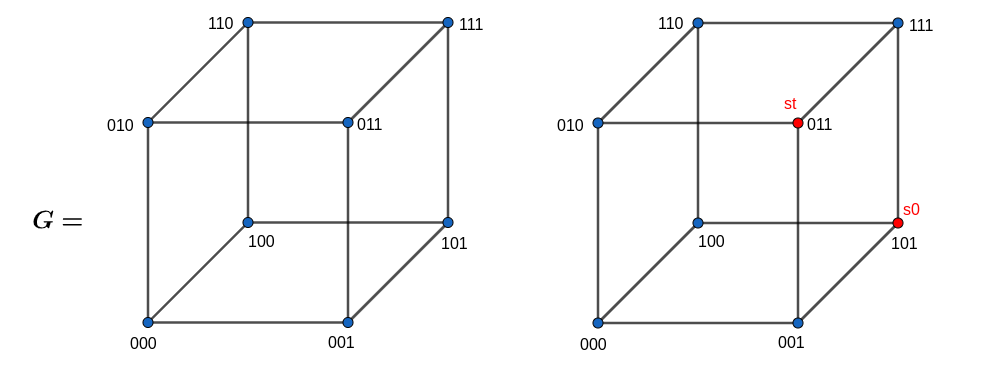
\includegraphics[width=0.8\textwidth]{res/hypercube.png}
\caption{left image:3-dimensional hypercube containing all possible assignments. Right image : two assignments satisfying $\phi$.}
\label{fig:circle}
\end{figure}
\end{example}

\subsubsection{Basic concepts and statements of results}
The first to analyze the connectivity properties of the configuration graphs of satisfiability problems were Gopalan et al. \cite{gopalan_connectivity_2006}. Their work is the continuity of Schaefer's work \cite{schaefer_complexity_1978}. The latter introduced a framework for expressing variants of Boolean satisfiability and a very well celebrated theorem called the Dichotomy theorem. 

\paragraph{Schaefer's framework}
\begin{defn}
A logical relation $\mathcal{R}$ is a non-empty subset of $\{T,F\}^{k}$ where $k$ is the arity of $\mathcal{R}$ for some $k \geq 1$. 

\begin{example}
If $\mathcal{R}_{1/3} = \{TFF,FTF,FFT\}$, then  $\mathcal{R}_{1/3}(x_1,x_2,x_3)$ is TRUE if and only if exactly one of $x_1$,$x_2$,$x_3$ is assigned to TRUE. 
\end{example}
\end{defn}

\begin{defn}
Let $\mathcal{S}$ be a finite set of logical relations. A  $CNF(\mathcal{S})-formula$ over a set of variables $V = \{x_1,x_2,\dots,x_n   \}$  is a finite conjunction $c_1 \wedge c_2 \wedge \dots \wedge c_m$ of clauses built using relations from $\mathcal{S}$. \\
Hence each $c_i$ is an expression of the form $\mathcal{R}(\varepsilon_1,\varepsilon_2,\dots,\varepsilon_k)$ where $\mathcal{R}$ is a logical relation and each $\varepsilon_j \in V or \{T,F\}$. A solution of a $CNF(\mathcal{S})-formula$ $\phi$ is an assignment $s = (s_1, \dots, a_n)$ of Boolean values to the variables that makes every clause of $\phi$ true. 
\end{defn}

\begin{defn}
The $SAT(\mathcal{S})$ problem associated with a finite set of logical relations $\mathcal{S}$ asks : 
Given a CNF($\mathcal{S}$)-formula $\phi$, is it satisfiable ?
\end{defn}

\begin{remark}
All well known restrictions of Boolean satisfiability problems, such as $3$-SAT, NOT-ALL-EQUAL $3$-SAT and POSITIVE $1$-IN-$3$SAT can be cast as SAT($\mathcal{S}$) problems, for a suitable choice of $\mathcal{S}$. 
\end{remark}

\begin{example}
Let $R_0 = \{0,1\}^{3} \backslash \{000\}$,
$R_1 = \{0, 1\}^{3} \backslash\{100\}$, $R_2 = \{0,1\}^{3} \backslash\{110\}$, $R_3 = \{0,1\}^{3} \backslash\{111\}$. Then $3-SAT$ is the $SAT(\mathcal{S})$ problem where $\mathcal{S} =   ({R_0 , R_1 , R_2 , R_3 })$. Similarly, POSITIVE 1- IN -3S AT is $SAT({R_{1/3}})$, where $R_{1/3} = \{100, 010, 001\}$.
\end{example}

\paragraph{Dichotomy theorem} \\ [breakline]
\\
Schaefer classified the Boolean constraint satisfaction problem and showed that, for certain sets $\mathcal{S}$, $SAT(\mathcal{S})$ is solvable in polynomial time while for all other sets $\mathcal{S}$ the problem is $\mathcal{NP}-complete$. \\ 
Schaefer gave $6$ classes for which $SAT(\mathcal{S})$ is solvable in polynomial and proved that all other sets of relations generate an $\mathcal{NP}$-complete problem. \\ 
A set $\mathcal{S}$ of logical relations is Schaefer if all relations in $\mathcal{S}$ are either bijunctive, Horn, dual Horn, or affine. \cite{schaefer_complexity_1978}

\paragraph{Tight relations class\cite{gopalan_connectivity_2006}}
The class of tight relations can be seen as a superset of Schaefer relations. Gopalan et al. were mostly interested about the reachability problem and thus created a dichotomy theorem analogous to Schaefer's.  

\begin{defn}
st-Conn($\mathcal{S}$) : Given a CNF($\mathcal{S}$)-formula $\phi$, and two satisfying assignments $s$ and $t$ of $\phi$,is there a path between $s$ and $t$ in the configuration graph of solutions of $\phi$?
\end{defn}

\begin{defn}
Conn($\mathcal{S}$)Given a CNF($\mathcal{S}$)-formula $\phi$, is the configuration graph of solutions of $\phi$ connected?
\end{defn}

\begin{theorem} \cite{DBLP:journals/corr/Heuvel13}
Let $\mathcal{S}$ be a finite set of logical relations.
\begin{enumerate}
    \item If $\mathcal{S}$ is tight, then st-Conn($\mathcal{S}$) is in $\mathcal{P}$; \\otherwise, st-Conn($\mathcal{S}$) is PSPACE-complete. 
    \item If $\mathcal{S}$ is tight, then Conn($\mathcal{S}$) is in coNP, \\if it is tight but not Schaefer, then it is coNP-complete; \\otherwise, it is PSPACE-complete.
    \item If every relation R in S is the set of solutions of a 2-CNF-formula, then
Conn(S) is in P.
\end{enumerate}
\end{theorem}

\begin{footnotesize}
Please refer to \cite{gopalan_connectivity_2006} for the formal definition of tight sets 
\end{footnotesize}


